\chapter{Introduction} 
\label{chapter1}

Advancements in sensing, perception, and low-cost embedded computing have resulted in the rapid growth of 
autonomous vehicle technology over the last two decades. Once the subject of sci-fi imagination in world exhibitions and 
popular journalism, semi-autonomous driving features such as emergency braking, autonomous lane guidance
and adaptive cruise control are now readily available. Furthermore, many automotive manufacturers
 and technology firms are developing automated vehicles requiring little or no human interaction \cite{hocky}\cite{alexdavies}\cite{iglauer}\cite{curtis}\cite{heatherkelly}\cite{mikeramsey}. 

The potential benefits of an automated vehicle ecosystem are significant. A comprehensive 2015 study by the consulting 
firm McKinsey and Company \cite{McK} estimates that widespread adoption of
autonomous vehicle technology would reduce automobile accidents by over 90\%, preventing thousands of fatalities, hundreds of
thousands of hospitalizations, and many billions of dollars in property damage annually.

While a large portion of autonomous vehicle research and development is focused on handling routine driving situations, achieving the safety benefits of
autonomous vehicles also requires a \textbf{focus on automated driving at the limits of tire friction}. The need for an automated vehicle to 
fully utilize its capability can arise when avoiding a collision with human-operated vehicles. This is crucial from an automotive safety
standpoint as human error accounts for over 90\% of automobile accidents \cite{bws}, and there will likely be a significant period of time where
autonomous vehicles must interact with human-operated vehicles \cite{McK}. Furthermore, successful handling at the friction limits will
be required where environmental factors are involved, such as unpredicted natural obstructions and poor tire friction caused by inclement weather (e.g. ice, rain). 
The potential for technology to assist in friction-limited situations has already been demonstrated by electronic stability control (ESC) systems, which reduced 
single-vehicle accidents by 36\% in 2007 \cite{jendang} and are now standard on all passenger cars. 

\section{Driving at the Handling Limits}

Each of the four tires on an automobile contacts the road surface over a contact patch, an area roughly the size of a human hand (Fig.~\ref{fig:basicPhysics}(b)). 
As shown in Fig.~\ref{fig:basicPhysics}(a), these contact patches generate the friction forces between the tire and road that are necessary for both vehicle longitudinal acceleration (braking and acceleration)
as well as lateral acceleration (turning). Because the available friction between the tire and road is limited, each of the four
tires is limited in the turning, braking, and accelerating forces they can produce. This relationship is given for each tire by the commonly known
``friction circle" equation: 

\begin{equation}
\mu F_z \geq \sqrt{F_x^2 + F_y^2}
\label{eq:fricCircle}
\end{equation}
where $\mu$ is the friction coefficient between the tire and the road, $F_z$ is the normal force acting on the tire, and $F_x$ and
$F_y$ are the lateral and longitudinal forces, respectively (Fig.~\ref{fig:basicPhysics}(c)). One key insight from (\ref{eq:fricCircle}) is that the cornering and
braking ability of the car is heavily determined by the amount of friction. On a dry, paved asphalt surface, values of $\mu$ are typically
equal to 1.0. However, on wet or rainy asphalt, $\mu$ can decrease to 0.7, and in snow or ice, the value of $\mu$ can be 
as low as 0.2 \cite{fricStudy}. Another insight from (\ref{eq:fricCircle}) is the coupled relationship between vehicle lateral and longitudinal forces. If the vehicle
is braking (or accelerating) heavily, the value of $F_x^2$ will be large and there will be less friction force available for turning. 

 \begin{figure}
\centering
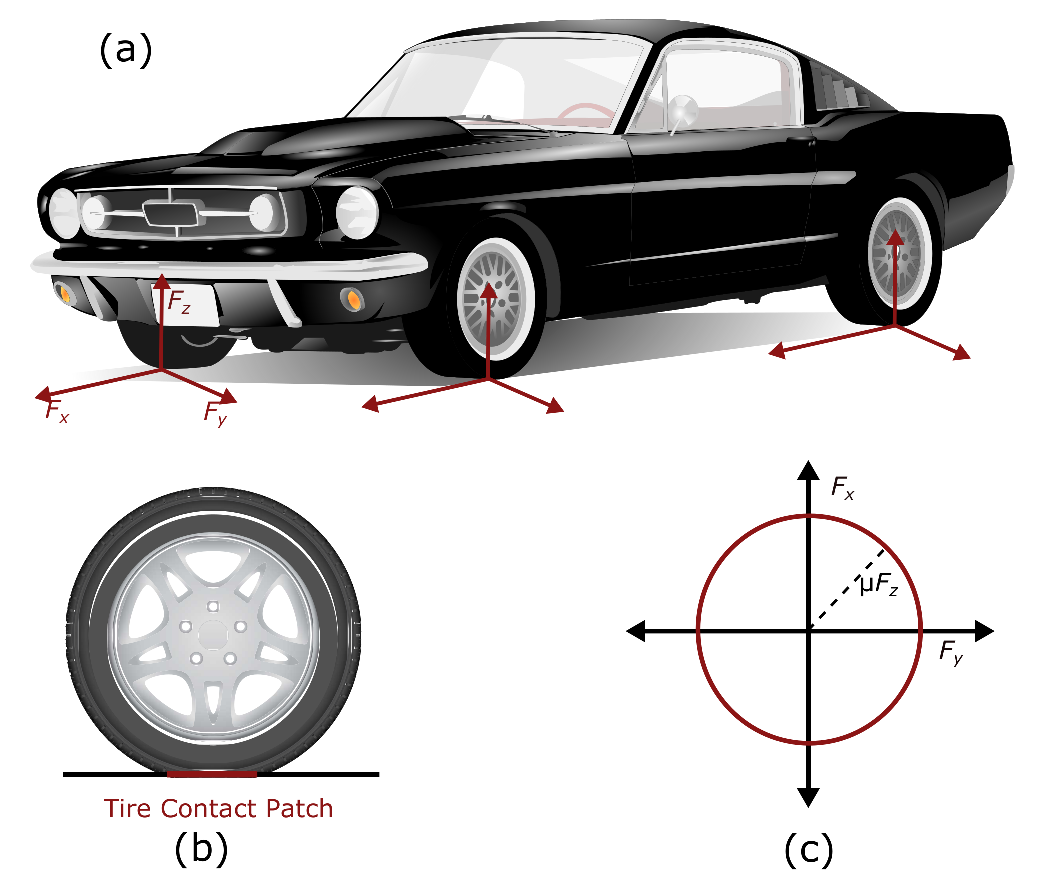
\includegraphics[width= \textwidth]{frictionForces.eps}
\caption[Driving at the limits]{(a) Friction forces $F_x$ and $F_y$ generated in the contact patch allow for lateral and longitudinal vehicle acceleration. (b)
Side view of tire contact patch. (c) Graph showing combined lateral and longitudinal force capability for a tire given the normal load
and friction coefficient $\mu$.}
\label{fig:basicPhysics}
\end{figure}

\subsection{Exceeding the Friction Limits: Understeer and \newline Oversteer}
\label{sec:osteerusteer}
In normal driving situations, the forces required for turning, braking, and accelerating will be much smaller than the
 available friction force. However, in rainy or icy conditions, accidents frequently occur when the driver enters a turn too fast
 or when the driver attempts to turn too quickly while already applying the brakes. In these situations, the tire forces at either the
 front or rear axle become saturated, resulting in one of two distinct scenarios. 

 When the front tires forces become saturated, the vehicle will \textit{understeer}, as illustrated in Fig.~\ref{fig:underover}(a).
 The steering actuator of a vehicle only has direct control of the front tire forces. As a result, 
 additional turning of the steering wheel will not generate additional lateral force or acceleration when the front axle is saturated.
The vehicle therefore becomes uncontrollable and has no ability to reduce the radius of its turn. 
  \begin{figure}[h]
\centering
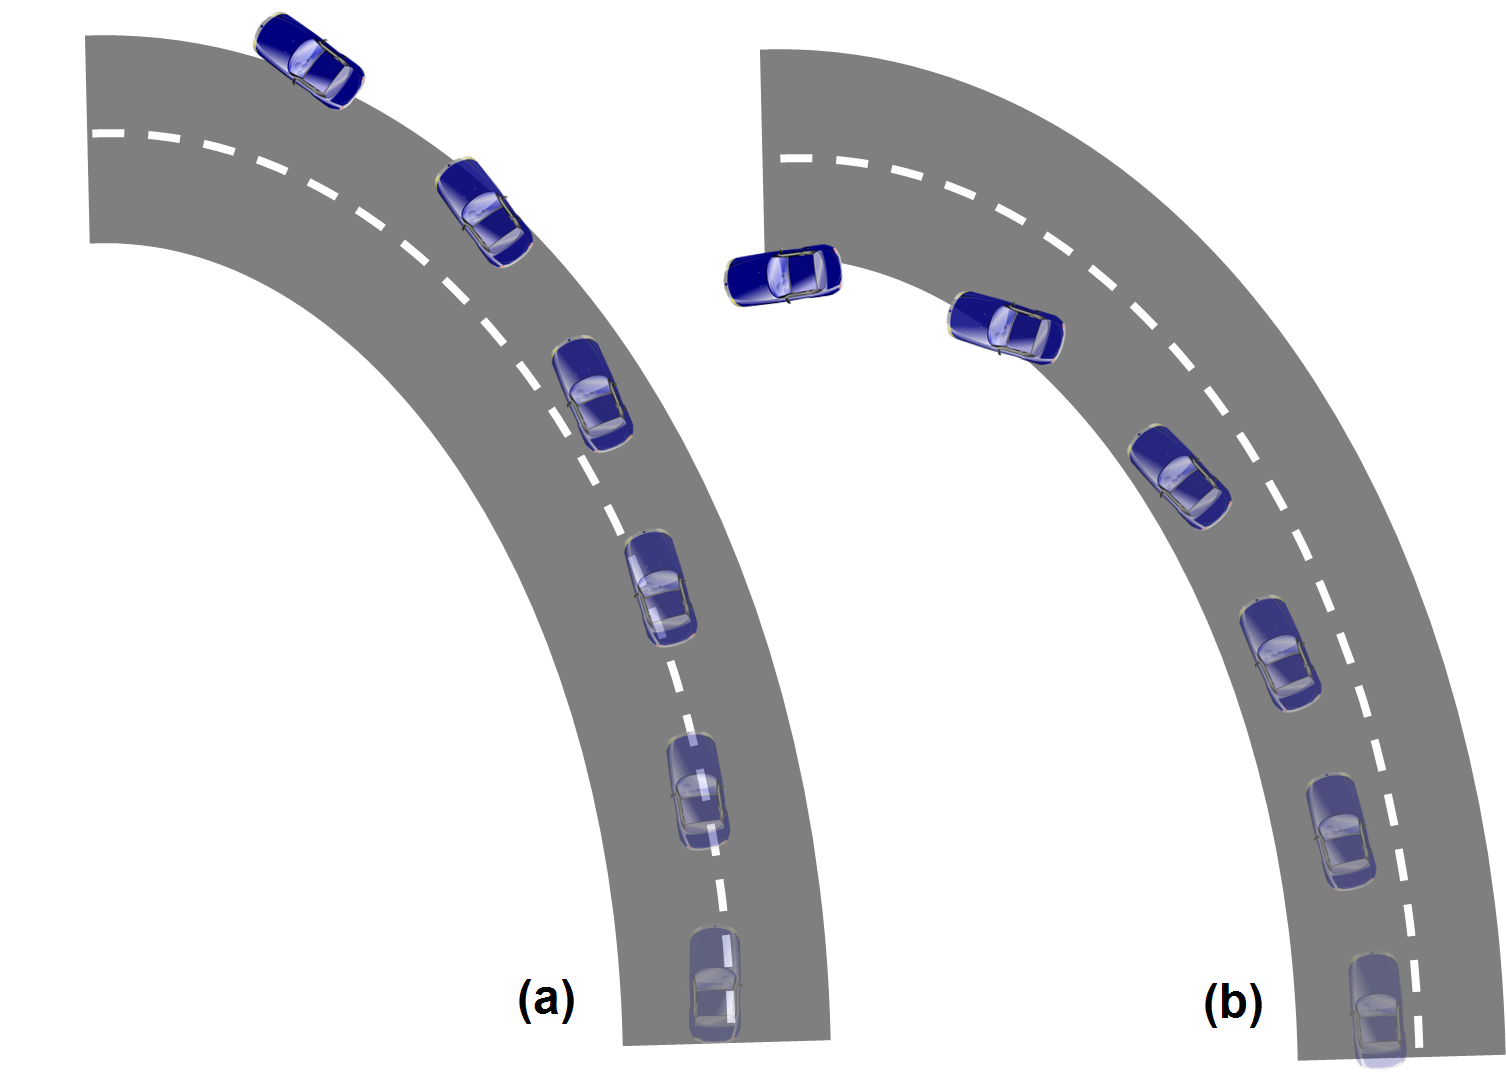
\includegraphics[width= .8\textwidth]{understeeroversteer.png}
\caption[Understeer and Oversteer]{(a) Vehicle understeering at the limits of handling. (b) Vehicle oversteering at the limits of handling.}
\label{fig:underover}
\end{figure}

For the converse scenario where the rear tire forces become saturated, the vehicle
 enters an \textit{oversteer} condition, as illustrated in Fig.~\ref{fig:underover}(b). In this situation, the vehicle loses stability and begins to
spin. An oversteer situation differs
 from an understeer because the front tire forces are not saturated, and the steering actuator can therefore be used to fully control the vehicle. As a result, it is possible
to apply a \textit{countersteer} maneuver to reverse the vehicle spin and gain control of the vehicle without deviating from the desired path.

 % Both conditions are extremely dangerous as they can easily result in the
 % vehicle colliding with a fixed obstacle such as a tree or with another vehicle. In large vehicles such as SUVs, understeer and oversteer
 % can also result in vehicle rollover. 
\section{Race Car Driving as Inspiration for \newline Autonomous Safety Systems}

Automotive engineers today face the challenge of designing autonomous safety systems that can utilize 
the full capabilities of the vehicle's tires in emergency scenarios to avoid accidents and
significant understeer or oversteer. While this is a difficult task, professional race driving provides a source of inspiration for 
designing autonomous safety systems. 

In order to complete a race in minimum time, race car drivers use nearly 100\% of the 
available friction between their vehicle's tires and the road. Professional drivers are extremely skilled at coordinating
 their brake, throttle, and steering inputs to maximize the speed of the vehicle through all corners of a race course while keeping
the vehicle tires within the friction limits. Furthermore, they must achieve this while avoiding collisions with
 other competing drivers who are also driving extremely aggressively. Finally, race car drivers often exceed the friction limits temporarily
 while seeking the fastest lap time, and have the ability to re-stabilize the vehicle from an understeer or oversteer scenario. 
 
\textbf{The primary focus of this dissertation is therefore to develop a set of control algorithms that allow an autonomous vehicle to drive at the handling limits with
the same capability as a professional race driver.} In particular, these algorithms focus on autonomously completing three primary tasks that race car drivers demonstrate with 
proficiency:

\begin{enumerate}
 		
  \item \textbf{Vehicle Steering at the Limits of Handling}. A vital task of racing is steering an automobile through a race course at the handling limits. Given the high lateral
  accelerations required for racing, mitigating vehicle oversteer or understeer is necessary. Good race car drivers have the ability to quickly and aggressively operate the
  steering wheel to complete a turn while maintaining vehicle stability.  
  
  \item \textbf{Finding a Time-Optimal ``Racing Trajectory"}. Given a race track and race vehicle, another fundamental task of racing is determining the fastest
		trajectory, or ``racing line" for the vehicle to follow. Race car drivers are skilled at driving though a race track along a path that enables them to take larger
		radius turns and accelerate aggressively on straight paths, increasing the permissible speed of the vehicle given tire friction constraints.
  
  \item \textbf{Lap-to-Lap Learning}. Finally, most races require the driver to complete many laps around the same race track. Given this repetition, 
	race car drivers have the opportunity to improve their lap times by slightly modifying their driving behavior on each lap to account for observations made during prior laps.
	The ability to learn from prior laps of driving also enables race car drivers to account for changing conditions (e.g. increasing temperatures, tire wear) over the course of a race.
  
\end{enumerate} 

While these tasks may seem specific to the niche field of race car driving, algorithms that enable a vehicle to autonomously drive like a race professional have 
enormous potential for vehicle safety systems. Algorithms that allow for steering at the limits of handling can be vital in piloting a vehicle through
a sudden stretch of icy road during the winter. With a small modification to the objective function, an algorithm that maximizes the turning radius on a race course can 
be used to maximize the distance between a vehicle and oncoming traffic. Learning algorithms that allow more precise driving over a fixed race course can be used to assist
drivers with their daily commute. Potential applications of the developed racing algorithms will be discussed further in the conclusion of this dissertation.

\section{State of the Art}
\label{sec:soa}

There has been significant prior work focused on autonomous steering control at the friction limits, time-optimal trajectory planning, and
iteration-based learning control. This section provides a brief overview of prior work that is relevant to the research contributions presented in this dissertation.

\subsection{Autonomous Race Vehicles}
\label{sec:arv}
Given the highly visible marketing opportunity provided by racing, 
several automotive companies have made notable attempts at racing-inspired 
automated driving. In 2008, BMW introduced the ``Track Trainer", which records race data
collected from a professional driver. To ``replay" the professional's driving autonomously,
the vehicle tracks the pre-recorded speed and racing line with a proportional-derivative
controller for throttle and brake and a dynamic programming algorithm for steering \cite{ttrain}. 
Using pre-recorded inputs allows the controller to naively account for nonlinear vehicle dynamics
at the handling limits, although this approach limits the flexibility of the controller to respond to unpredicted events. 

A second German luxury brand, Audi AG, also launched a collaborative research effort with Stanford University in 2008. 
The collaboration, with which this doctoral research is affiliated, resulted in the development of ``Shelley", an autonomous Audi TTS. Doctoral work by Stanford
 students Theodosis \cite{paulthesis} and Kritayakirana \cite{mickthesis} provided initial forays into 
 racing line generation and trajectory-following algorithms. Notable early accomplishments include autonomous driving
at speeds of 190 mph at the Salt Flats in Utah and an autonomous drive up the Pikes Peak International Hill Climb in 2009 \cite{ppeak}\cite{saltflats}. 
More recently, Audi has incorporated results from the collaboration to build a demonstration vehicle for media events, ``Bobby" (Fig.~\ref{fig:bobby}), 
an autonomous RS7 which debuted at Germany's Hockenheimring \cite{hocky}. The primary focus for the RS7 vehicle was robustness,
enabling the vehicle to be demonstrated at a public event with journalists inside the vehicle at high speeds. 	

 \begin{figure}
\centering
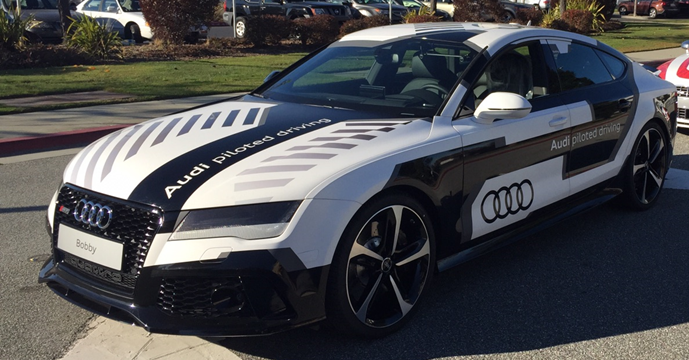
\includegraphics[width= .75\textwidth]{bobby.png}
\caption[Audi's autonomous RS7]{``Bobby", Audi's autonomous RS7.}
\label{fig:bobby}
\end{figure}
 
\subsection{Automated Steering at the Limits of Handling}
\label{pw1}

In the 1990's and early 2000's, a primary focus of autonomous driving research was
designing control systems to follow a desired path \textit{below} the limits of handling. Initial designs typically centered
around linear feedback-feedforward controllers, using linear models of the vehicle dynamics to design the steering control laws \cite{shladover}. An
important development at this time was the idea of \textit{lookahead} steering feedback, where the objective is to 
minimize the lateral tracking error at a certain point in front of the vehicle \cite{guldner}\cite{hingwe}\cite{rosseter}. 

Given the success of linear controller designs for automated steering, early 
attempts at driving at the handling limits also made the assumption of linear vehicle dynamics. While the dynamics of an 
automobile become nonlinear at the handling limits due to tire saturation, assuming linear dynamics in the controller design 
resulted in respectable results in several studies \cite{bessyboy}\cite{sharpysharp}\cite{tommyboy}. To improve upon these results, 
more recent publications have proposed control systems that account for the nonlinear effect of tire saturation at the handling limits
\cite{filho14}\cite{mickcop}\cite{yang14}. The most recent development has been the application of model-predictive control (MPC), which enables
state-of-the-art steering controllers to track a path at the handling limits while trading off between competing objectives of obstacle avoidance and vehicle stabilization \cite{carvalho13}\cite{joethesis}.

While there are a wide variety of published steering controllers with varying levels of complexity, there is no single experimentally validated
controller that displays a well-understood combination of robust stability margins and low path tracking error both at the limits of handling and
in ordinary driving situations. Work by
 Rosseter \cite{rosseter} and Talvala \cite{talvthesis} provides great analysis of the
desirable stability properties of lookahead steering feedback, but no discussion of how path tracking behavior changes as the
vehicle approaches the limits of handling. Kritayakirana and Gerdes \cite{mickcop} 
presented a steering controller with lookahead feedback and a feedforward designed to provide zero lateral error at the vehicle \textit{center of percussion}, a special point within the vehicle frame. 
This method was validated experimentally at the limits of handling and had desirable stability properties, although there was an
issue of competing feedback and feedforward control due to the selection of inconsistent error minimization points. 
Experimentally validated results using model-predictive control \cite{carvalho13}\cite{joethesis} demonstrate the ability to balance competing
objectives of vehicle path tracking and stability when the front or rear tires are saturated, but 
consist of complex optimization problems that make fundamental issues such as stability and closed-loop tracking performance difficult to analyze mathematically or
understand qualitatively. 

\subsection{Time-Optimal Trajectory Planning}
\label{pw2}

The problem of calculating the minimum lap time trajectory for a given vehicle and race track has been studied over the last several decades
in the control, optimization, and vehicle dynamics communities. Early attempts were generally focused on determining analytical
solutions for simple maneuvers via the calculus of variations \cite{hendrikx} or developing qualitative insights for race car drivers and enthusiasts \cite{mken}\cite{taruffi}. With advances in computing power and numerical optimization techniques, 
minimum-time path planning sparked the interest of professional racing teams hoping
to quantitatively determine the effect of vehicle modifications on the optimal lap time for a specific racing circuit. Casanova \cite{casanova} therefore developed a method in 2000 (later 
refined by Kelly \cite{kelly} in 2008) capable of simultaneously optimizing both the path and speed profile
for a fully nonlinear vehicle model using nonlinear programming (NLP). The developed software helped Formula One race teams
analyze the effects of subtle changes in vehicle parameters, including tire thermodynamic properties and suspension designs.

More recently, the development of autonomous vehicle technology has led to research on optimal path
 planning algorithms that can be used for driverless cars. Theodosis and Gerdes published a nonlinear gradient descent approach for determining time-optimal racing lines
 \cite{theodosis}, which has the rare distinction of being validated experimentally on an autonomous race vehicle. 
  
 However, a significant drawback of nonlinear programming solutions is high computational expense. Given the need for real-time trajectory planning in
 autonomous vehicles, there has been a recent interest in finding approximate methods that provide fast lap times with low computational expense. Published methods include formulating the minimum lap time problem
 into a model predictive control (MPC) problem \cite{morari}\cite{timings} or solving a series of locally optimal optimization
 problems \cite{gerdts}\cite{velly}. However, one potential 
 drawback of the model predictive control approach is that an optimization
 problem must be reformulated at every time step, which can still be computationally expensive.
 
 Experimental validation on an 
 autonomous race vehicle has only been reported by Theodosis and Gerdes \cite{theodosis} and Gerdts et al. \cite{gerdts}. 
 To the author's knowledge, a trajectory planning algorithm with a runtime close enough for real-time implementation has not been validated on an experimental vehicle.
 While an autonomous vehicle can apply a closed-loop controller to follow a time-optimal vehicle trajectory computed offline,
 there are  significant benefits to developing a fast trajectory generation algorithm that can approximate the globally optimal trajectory in real-time. 
 If the algorithm runtime is small compared to the actual lap time, the algorithm can run as a real-time trajectory planner and find a fast racing line 
 for the next several turns of the racing circuit. This would allow the trajectory planner to modify the desired path based on the motion of competing race vehicles and 
 estimates of road friction, tire wear, engine/brake dynamics and other parameters learned over several laps of racing. Additionally, the fast trajectory algorithm can
 be used to provide a very good initial trajectory for a nonlinear optimization method.  

\subsection{Iteration-Based Learning}

Developing algorithms that mimic a human's ability to adapt and learn over time has been a focus for researchers in a variety
of fields. In the field of automated control, an interesting approach for adaptation is iterative learning control (ILC), based
on the notion that the performance of a system that executes the
\textit{same task} multiple times can be improved by learning from previous executions \cite{bristow}.
Because iterative learning control works best when learning to follow the same reference trajectory under the same ambient conditions, the most common applications
of ILC are in the field of automated manufacturing. Notable examples include CNC machining \cite{kimdi}, industrial robotics \cite{freeman}\cite{hladowski}, piezolectric stage
positioning \cite{huang}, motor control \cite{mohammad}, and microdeposition \cite{hoelzle}. However, the rise of automated systems outside
factory environments has led to preliminary applications of ILC for ground and air robotics \cite{chen}\cite{purwin}\cite{sun}.

 In the field of computer science, a technique widely used for training in automated systems is \textit{reinforcement learning}.
 Reinforcement learning is similar to iterative learning control in that an automated system overcomes uncertainty in the world by
 gradually learning over multiple trials. However, iterative learning control algorithms typically assume the system is modeled by a 
 discrete (often linear) dynamic system, with uncertainty in the form of an unknown but repeating disturbance. On the other hand, 
 reinforcement learning algorithms act on systems modeled by Markov Decision Processes (MDPs), with the uncertainty typically in
 the form of unknown state transition probabilities and rewards. Furthermore, iterative learning algorithms attempt to gradually
 determine an input \textit{control signal} to overcome the unknown disturbance and provide accurate tracking of a reference trajectory. 
 Reinforcement learning algorithms are more general, and develop a \textit{policy} that maps any state within the MDP to
 an optimal action. 

 Like recent ILC research, reinforcement learning has also been widely investigated for applications in ground and air robotics. 
 In the field of UAV control, Ng et al. presented a reinforcement learning algorithm to learn
a controller for autonomous inverted helicopter flight \cite{ng2006}. There have also
been many publications in the area of robotic motion control. For example, in a modification
of reinforcement learning known as ``apprenticeship learning" Lee et al. presented research
where a robot was able to tie a knot after observing human-guided observations \cite{abbeel}. Finally, in the
area of autonomous vehicles, Lauer presented a reinforcement learning approach to designing a steering
controller for a 1:5 scale RC car \cite{lauer}.

In summary, iteration-based learning algorithms have a rich history of validation on manufacturing and robotic systems. Developing similar
algorithms for an autonomous race vehicle could therefore yield significant benefits. Even with a well-designed trajectory planner
 and path-following controller, there will often be regions of the race track where transient vehicle
 dynamics and unmodeled disturbances result in poor tracking of the optimal trajectory. Furthermore, a major determinant of the 
 optimal trajectory is the friction coefficient between the road and the tires. In reality, this is hard to know ahead
of time beyond a reasonable estimate (e.g $0.95 \leq \mu \leq 1.0$). However, at the limits of handling, small differences in the amount of grip
between the tires and road can result in significant lap time differences. Additionally, turns before a long straight section of track
must be driven more cautiously than series of consecutive turns, because exceeding the friction limit can result in lower top speeds
on the fastest part of the track, significantly increasing lap times. Human drivers
understand this effect well, especially for front-heavy vehicles, and use the term ``slow-in, fast-out" to describe their strategy on crucial turns
before a long straight section. The difficulty of precisely following a racing trajectory at the handling limits and determining the optimal acceleration limits
points to the need for a learning approach that can improve lap time performance over multiple laps of driving.
 
\section{Research Contributions and Outline}
Section \ref{sec:soa} provided a brief overview of the state of the art for the three primary tasks of trajectory planning, trajectory following and
iteration-based learning. Opportunities for important further research in each task were articulated as well. 
This section outlines the primary contributions of this doctoral work for each of these racing-inspired research areas. 

\subsubsection{Chapter 2: A Feedback-Feedforward Steering Controller for Accurate Path Tracking and Stability at the Limits of Handling}

Chapter 2 of this dissertation presents a feedback-feedforward steering controller that maintains vehicle stability at the handling limits
along with strong path tracking performance where physically possible. The design begins by considering the performance of a baseline
controller with a lookahead feedback scheme and a feedforward algorithm based on a nonlinear vehicle handling diagram.
While this initial design exhibits desirable stability properties 
at the limits of handling, the steady-state path deviation increases significantly at highway speeds. 
Results from both linear and nonlinear analyses indicate that lateral path tracking deviations are minimized when vehicle sideslip 
is held tangent to the desired path at all times. Analytical results show that 
directly incorporating this sideslip tangency condition into the steering feedback dramatically improves lateral path tracking, 
but at the expense of poor closed-loop stability margins.  However, incorporating the desired sideslip behavior
into the feedforward loop creates a robust steering controller capable of accurate path 
tracking and oversteer correction at the physical limits of tire friction. Experimental data collected from an 
Audi TTS test vehicle driving at the handling limits (up to 9.5 $\mathrm{m/s^2}$) on a full length race circuit demonstrates the
 improved performance of the final controller design. 

\subsubsection{Chapter 3: A Sequential Two-Step Algorithm for Fast Generation of \newline Vehicle Racing Trajectories}
 \label{ch1FGbenefits}
  
 Chapter 3 presents an iterative algorithm that divides the path generation
 task into two sequential subproblems that are significantly easier to solve than the fully nonlinear lap time optimization. Given an initial path through the race track, the algorithm
 runs a forward-backward integration scheme to determine the minimum-time longitudinal speed profile, subject to
 tire friction constraints. With this speed profile fixed, the algorithm updates the vehicle's path by solving a convex optimization problem 
 that minimizes the curvature of the vehicle's driven path while staying within track boundaries and obeying affine, time-varying vehicle dynamics constraints.
 This two-step process is repeated iteratively until the
 predicted lap time no longer improves. While providing no guarantees of convergence or a globally optimal solution, 
 the approach performs very well when validated on the Thunderhill Raceway
 course in Willows, CA. The predicted lap time converges after four to five iterations, with each iteration over the full 4.5 km race course requiring
 only thirty seconds of computation time on a laptop computer. The resulting trajectory is experimentally driven at the race circuit with
 an autonomous Audi TTS test vehicle, and the resulting lap time and racing line are comparable to both a nonlinear gradient
 descent solution and a trajectory recorded from a professional racecar driver. The experimental results indicate that the proposed method is a viable option for 
 online trajectory planning in the near future.
 
 \subsubsection{Chapters 4 and 5: Iterative Learning Algorithms to Improve Autonomous Driving Performance}
 
This dissertation proposes two sets of learning algorithms that gradually refine the driving performance of the autonomous race car 
over time. Chapter 4 presents an iterative learning control (ILC) formulation to gradually determine the proper steering 
and throttle input for transient driving maneuvers along the race track. Racing is an ideal scenario for ILC because race cars 
drive the same sequence of turns while operating near the physical limits of tire-road friction. 
This creates a difficult to model, but repeatable, set of nonlinear vehicle dynamics and road conditions from lap to lap. 
Simulation results are used to design and test convergence of both a 
 proportional-derivative (PD) and quadratically optimal (Q-ILC) iterative learning controller, and 
experimental results are presented at combined vehicle accelerations 
of up to 9 $\mathrm{m/s^2}$.

Chapter 5 focuses on determining the best value of the friction coefficient $\mu$ for turn-by-turn trajectory planning on the track. Because
the friction coefficient is directly linked to the peak accelerations of the speed profile, locally varying $\mu$ for each turn on the track is a way
to tune the aggressiveness of the planned trajectory. Rather than directly encoding the ``slow-in, fast-out" heuristic that human drivers
typically employ, a learning approach is used to automatically determine the fastest strategy. A small but significant collection of data is gathered
from the autonomous vehicle driving different turns of the track with different values of $\mu$ assumed. From this data, an A* search algorithm
is devised that searches through the data and finds the best value of $\mu$ for each portion of the track in order to globally minimize the resulting
lap time. Key developments of this algorithm include designing an appropriate A* heuristic to minimize the needed computation time and designing the cost
function to account for the physical difficulty of altering the vehicle's trajectory while understeering or oversteering. 


%%% REMOVED FIGURES %%%

 % \begin{figure}
% \centering
% \includegraphics[width= \textwidth]{cars.png}
% \caption[Autonomous vehicle prototypes]{Top two rows: Autonomous vehicle prototypes from the top six global automotive manufacturers by volume. From top left: Toyota, General Motors, Hyundai, Ford, Volkswagen, Nissan. Bottom row:
% prototypes from three non-manufacturers. From left: Automotive suppliers Delphi and Bosch, technology firm Google. Images available from Google Search.}
% \label{fig:autoCars}
% \end{figure}

 % \begin{figure}[h]
% \centering
% \includegraphics[width= \textwidth]{adoptCurve.png}
% \caption[Possible adoption curve for autonomous vehicles]{Possible adoption curve for autonomous vehicles as proposed by Bertoncello and Wee \cite{McK}. There will likely be a significant
% period of time where autonomous vehicles must interact with human-operated vehicles.}
% \label{fig:adoptCurve}
% \end{figure}

 % \begin{figure}[h]
% \centering
% \includegraphics[width= \textwidth]{emergency.png}
% \caption[Possible emergency scenarios for autonomous vehicles]{Possible emergency scenarios requiring autonomous vehicle handling near the limits of tire friction, both for a multi-car
 % and single-car scenario. (a) Suddenly oncoming traffic caused by driver error could require an emergency maneuver at the limits of handling.
 % (b) A patch of ice on the road or other inclement conditions could lead to a rapid decrease in tire friction, quickly bringing an autonomous vehicle to the limits of handling.}
% \label{fig:emergency}
% \end{figure}